\clearpage
\subsection{Public Path: selección y publicación}\label{sec:publicacion}
\subsubsection{Valparaíso}
Par elegido: ICMP, ronda 3. Unión de 15 IP; 0 TTL sin respuesta en conjunto. Ida 227979504; vuelta 227979545.

UUID: 0d24e9fd-d1b3-11f1-be0a-005056ae3c32

\noindent\url{https://www.ndexbio.org/viewer/networks/0d24e9fd-d1b3-11f1-be0a-005056ae3c32}\par\medskip
\Needspace{9cm}
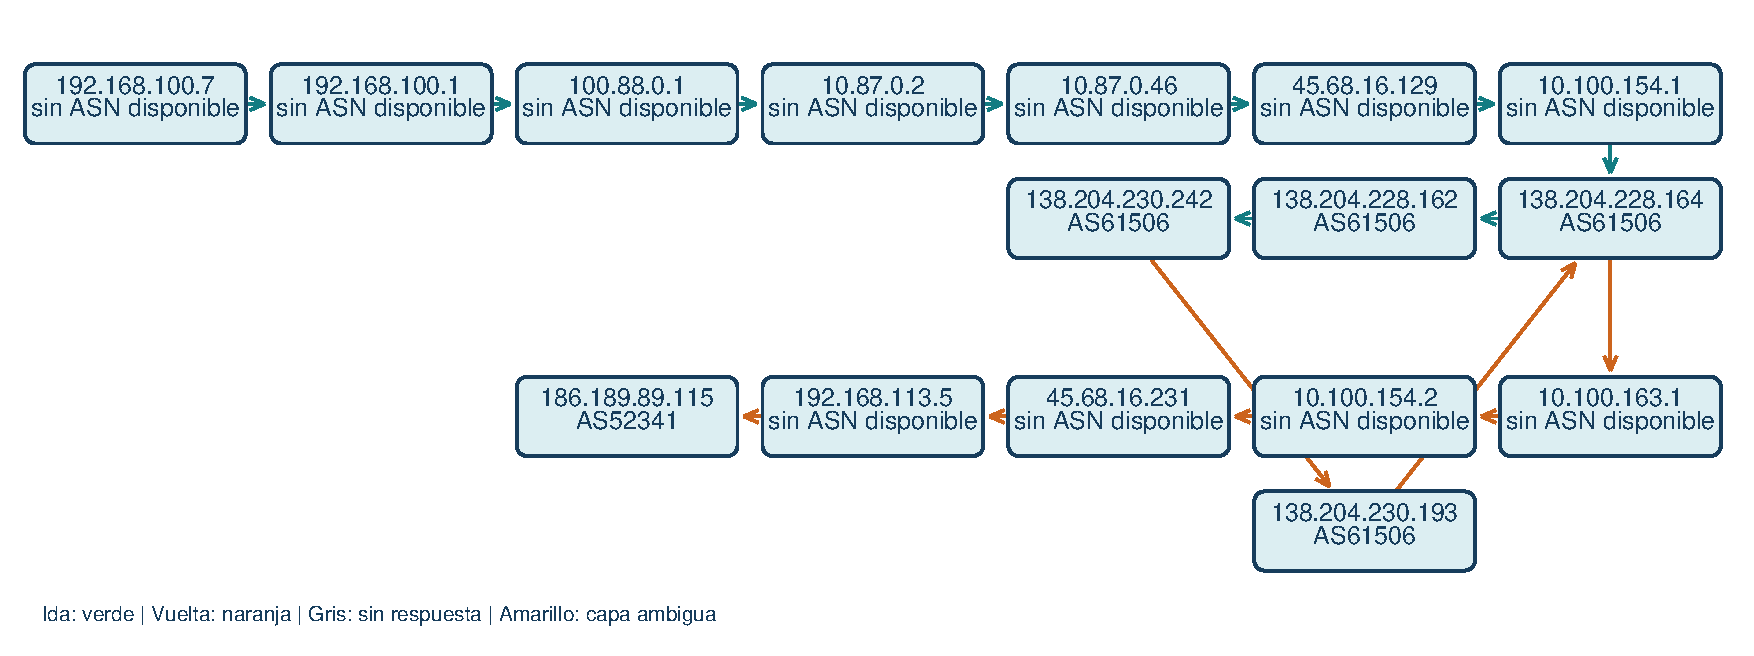
\includegraphics[width=\linewidth,keepaspectratio]{figuras/grafo_138.204.230.242.pdf}
\captionof{figure}{Representación vectorial del mismo CX2 publicado, Valparaíso. Las flechas indican sentido y las aristas son inferidas. }\label{grafo:138.204.230.242}
\subsubsection{La Habana}
Par elegido: TCP, ronda 2. Unión de 26 IP; 9 TTL sin respuesta en conjunto. Ida 227953132; vuelta 227953345.

UUID: fa23a62a-d1b2-11f1-be0a-005056ae3c32

\noindent\url{https://www.ndexbio.org/viewer/networks/fa23a62a-d1b2-11f1-be0a-005056ae3c32}\par\medskip
\Needspace{9cm}
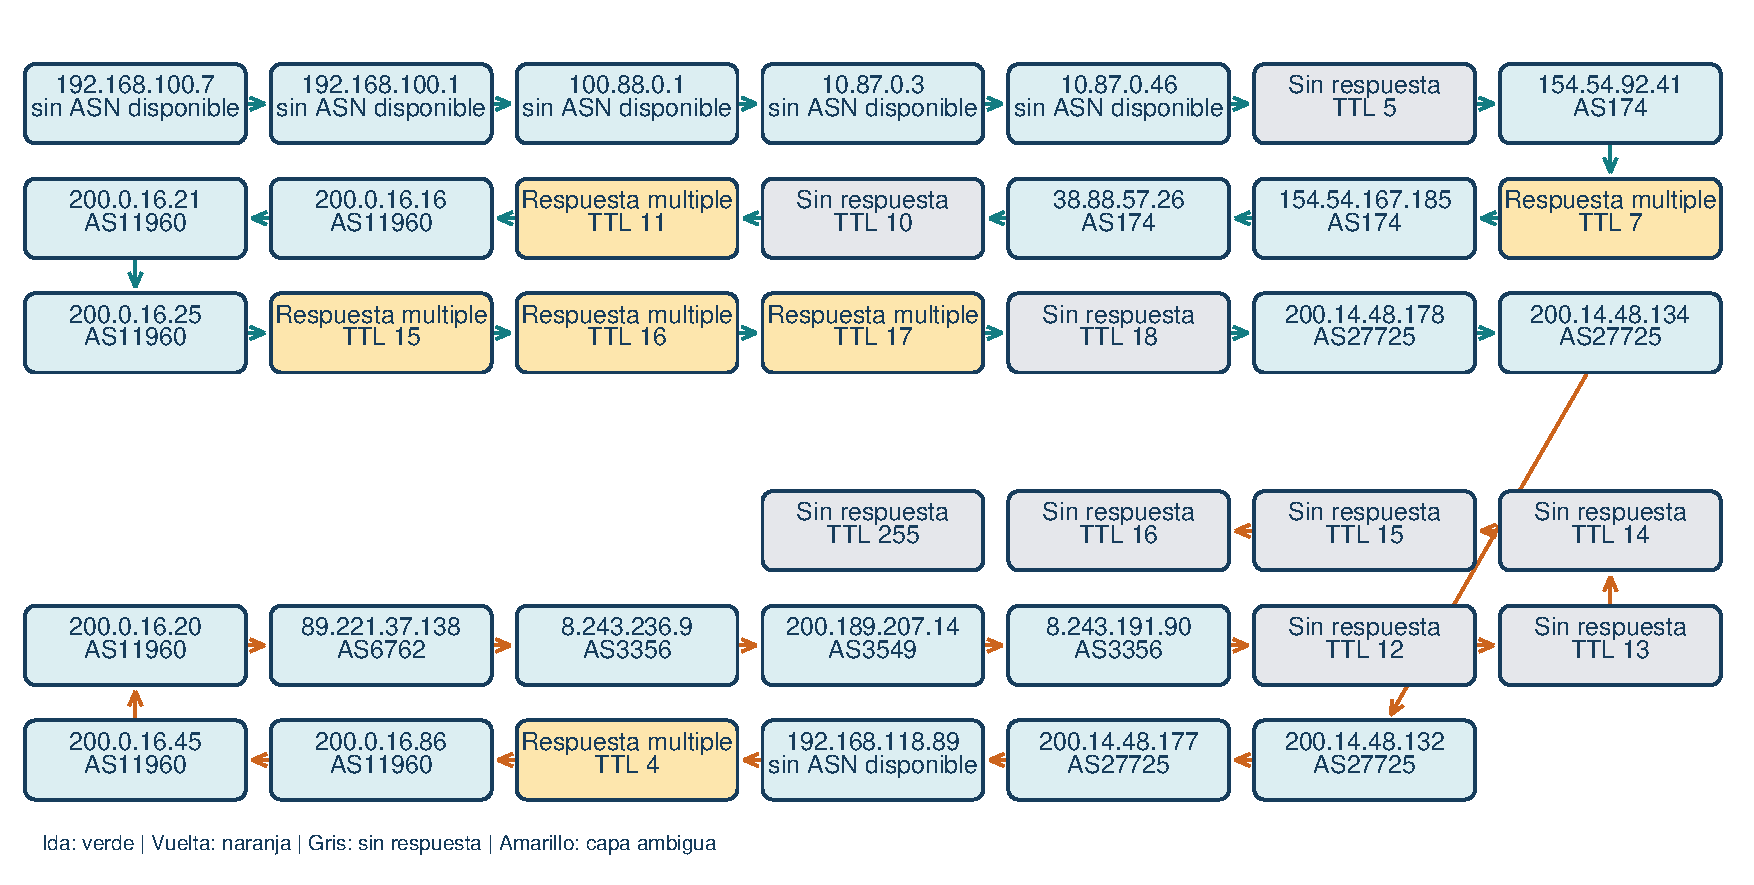
\includegraphics[width=\linewidth,keepaspectratio]{figuras/grafo_200.14.48.134.pdf}
\captionof{figure}{Representación vectorial del mismo CX2 publicado, La Habana. Las flechas indican sentidoy  las aristas son inferidas. }\label{grafo:200.14.48.134}
\subsubsection{Rusia}
Par elegido: ICMP, ronda 3. Unión de 20 IP; 4 TTL sin respuesta en conjunto. Ida 228276628; vuelta 228277013.

UUID: 6f78f82e-d219-11f1-be0a-005056ae3c32

\noindent\url{https://www.ndexbio.org/viewer/networks/6f78f82e-d219-11f1-be0a-005056ae3c32}\par\medskip
\Needspace{9cm}
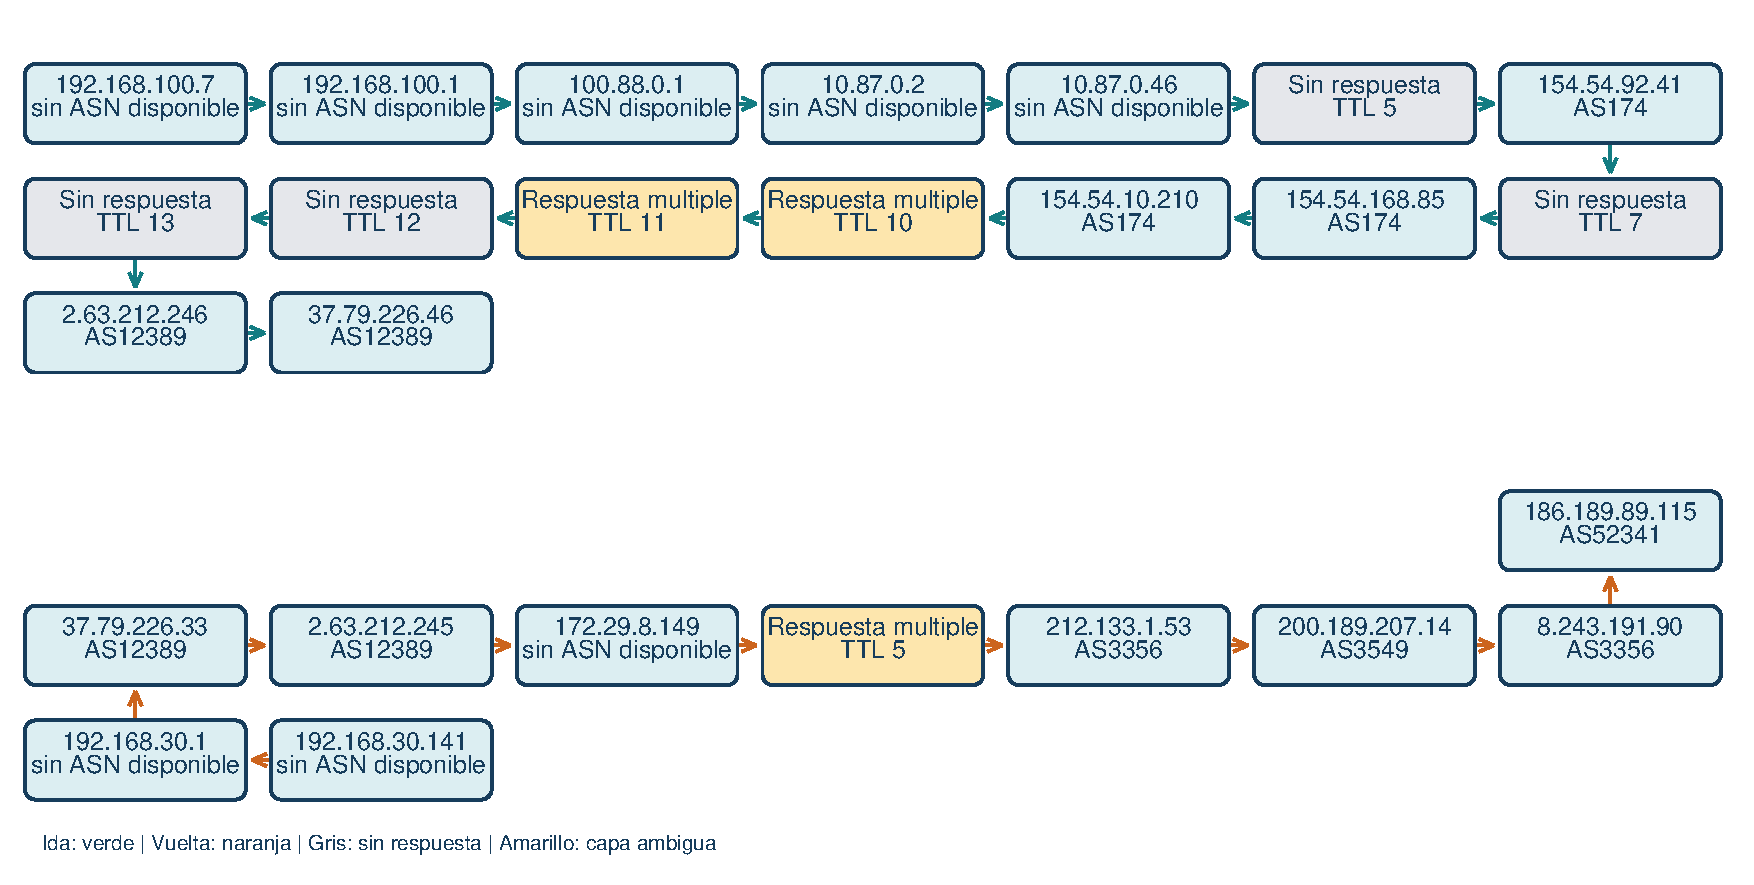
\includegraphics[width=\linewidth,keepaspectratio]{figuras/grafo_37.79.226.46.pdf}
\captionof{figure}{Representación vectorial del mismo CX2 publicado, Rusia. Las flechas indican sentido y las aristas son inferidas.}\label{grafo:37.79.226.46}
